\documentclass[conference]{IEEEtran}
\IEEEoverridecommandlockouts
% The preceding line is only needed to identify funding in the first footnote. If that is unneeded, please comment it out.
%Template version as of 6/27/2024
\usepackage{amsmath,amsfonts}
\usepackage{stmaryrd}
\usepackage{hyperref}
\hypersetup{colorlinks=true,citecolor = blue}
\newcommand{\Spt}{\texttt{Spt}}
\newcommand{\Rec}{\texttt{Rec}}
\newcommand{\DEnc}{\texttt{DEnc}}
\newcommand{\PEnc}{\texttt{PEnc}}
\usepackage[ruled,vlined,linesnumbered]{algorithm2e}
\usepackage{algorithmic}
\usepackage{booktabs}
\usepackage{multirow}
\usepackage{subfigure}
\usepackage{changepage}
\usepackage{cite}
\usepackage{amsmath,amssymb,amsfonts}
\usepackage{algorithmic}
\usepackage{graphicx}
\usepackage{textcomp}
\usepackage{xcolor}
\def\BibTeX{{\rm B\kern-.05em{\sc i\kern-.025em b}\kern-.08em
    T\kern-.1667em\lower.7ex\hbox{E}\kern-.125emX}}
\begin{document}

\title{MIND: A Privacy-Preserving Model Inference Framework via End-Cloud Collaboration*\\
{\footnotesize \textsuperscript{*}Note: Sub-titles are not captured for https://ieeexplore.ieee.org  and
should not be used}
\thanks{Identify applicable funding agency here. If none, delete this.}
}

\author{\IEEEauthorblockN{1\textsuperscript{st} Given Name Surname}
\IEEEauthorblockA{\textit{dept. name of organization (of Aff.)} \\
\textit{name of organization (of Aff.)}\\
City, Country \\
email address or ORCID}
\and
\IEEEauthorblockN{2\textsuperscript{nd} Given Name Surname}
\IEEEauthorblockA{\textit{dept. name of organization (of Aff.)} \\
\textit{name of organization (of Aff.)}\\
City, Country \\
email address or ORCID}
\and
\IEEEauthorblockN{3\textsuperscript{rd} Given Name Surname}
\IEEEauthorblockA{\textit{dept. name of organization (of Aff.)} \\
\textit{name of organization (of Aff.)}\\
City, Country \\
email address or ORCID}
\and
\IEEEauthorblockN{4\textsuperscript{th} Given Name Surname}
\IEEEauthorblockA{\textit{dept. name of organization (of Aff.)} \\
\textit{name of organization (of Aff.)}\\
City, Country \\
email address or ORCID}
\and
\IEEEauthorblockN{5\textsuperscript{th} Given Name Surname}
\IEEEauthorblockA{\textit{dept. name of organization (of Aff.)} \\
\textit{name of organization (of Aff.)}\\
City, Country \\
email address or ORCID}
\and
\IEEEauthorblockN{6\textsuperscript{th} Given Name Surname}
\IEEEauthorblockA{\textit{dept. name of organization (of Aff.)} \\
\textit{name of organization (of Aff.)}\\
City, Country \\
email address or ORCID}
}

\maketitle

\begin{abstract}
Image processing and analysis capabilities have been revolutionized by the rapid advancement of deep learning technologies. Complex neural networks, however, often demand computational resources that exceed those available on end-user devices. This limitation has led to the widespread adoption of cloud-based image inference, where resource-intensive computations are offloaded to powerful cloud servers.Although cloud servers help alleviate the resource constraints of these devices, transferring image data between the end device and the cloud is associated with high computational costs and significant privacy risks. Furthermore, traditional collaborative inference encryption methods typically involve directly encrypting image data, but this approach often fails to efficiently balance security and performance. To this end, in this paper, we propose a novel cloud-based collaborative encryption method called MIND, designed to enhance computational efficiency and reduce communication overhead. MIND divides the encryption process into two parts: model parameter encryption and image data encryption, applying these techniques to different layers of a neural network. Specifically, the end device encrypts part of the model parameters, while the cloud server encrypts the image data and the remaining model parameters. Our experiments show that MIND effectively balances usability with privacy protection.
\end{abstract}

\begin{IEEEkeywords}
Homomorphic encryption, Secret sharing, Hierarchical Encryption, Privacy protection.
\end{IEEEkeywords}

\section{Introduction}
Artificial intelligence and cloud computing advancements have revolutionized image processing and analysis capabilities across various industries \cite{makridakis2017forthcoming} \cite{zhang2010cloud}. The integration of deep learning models with cloud infrastructure has enabled unprecedented levels of visual data interpretation, from medical imaging to autonomous vehicle navigation. Within this technological landscape, cloud-based image inference techniques have gained significant traction, offering solutions to scenarios requiring efficient and secure processing of visual data \cite{shokri2017membership}. This shift towards cloud-powered image analysis has dramatically enhanced the ability to extract meaningful insights from vast amounts of visual information, while simultaneously raising important questions about data privacy and security.The widespread adoption of cloud computing compels users to provide their data to technical agencies in order to access corresponding services \cite{wang2018stealing}. For instance, certain residential areas may mandate the use of facial recognition gate systems, requiring residents to utilize their facial data as the sole method for entering and exiting the community \cite{cui2018security}. Similarly, the financial services industry may collect and analyze users' image information for commercial purposes without obtaining consumer consent. Given that these data contain sensitive personal information, such practices clearly fail to meet users' expectations for data protection. On one hand, we aspire to leverage new technologies to enhance our quality of life; on the other hand, we are unwilling to compromise our personal privacy. Therefore, additional measures must be implemented to safeguard the privacy and security of data \cite{van2014datafication}.

In cloud computing environments, model inference typically relies on the processing and analysis of large volumes of data, which often involves sensitive information \cite{fu2020vfl}. If these data are not effectively protected during transmission and storage, it can lead to data breaches \cite{yang2012efficient}. While traditional encryption methods can provide a certain level of data security, they also introduce substantial computational overhead and communication costs \cite{kerschbaum2012outsourced}. This issue is particularly evident when handling large-scale data, where the use of traditional encryption methods can result in inefficiencies \cite{li2015encdb}. To address these challenges, we propose MIND, a privacy-preserving model inference framework enabled by edge-cloud collaboration. By employing advanced encryption technologies such as homomorphic encryption and secret sharing, MIND ensures the security of data and model parameters during the inference process. By distributing computational tasks between edge devices and cloud servers, MIND can maintain the efficiency of model inference while protecting data privacy and reducing communication overhead. Within the MIND framework, we introduce a layered encryption scheme that dynamically adjusts encryption methods based on the model's structure, significantly reducing both computational and communication overhead. This innovative approach not only enhances system efficiency but also effectively safeguards data security without compromising model inference performance. MIND offers a practical privacy-preserving solution for model inference in cloud computing environments, striking a balance between privacy, security, and efficiency. This demonstrates its potential in future data encryption and privacy protection technologies.

\subsection{Contribution}

The conventional approach to image analysis typically involves encrypting the entire image before uploading it to the cloud server. However, this method results in significant storage and communication overhead, as the size of the encrypted images can be quite large. Additionally, conducting image analysis during transmission presents considerable privacy protection challenges, as sensitive data must be securely handled to prevent unauthorized access. Existing schemes exhibit deficiencies in several areas, including communication convenience, storage overhead, and privacy protection. These shortcomings can impede the practicality and effectiveness of image processing operations, particularly in scenarios involving large-scale data transmission and storage. To address these issues, we propose a novel approach designed to mitigate the computational burden caused by directly encrypting images transmitted by multiple parties. Our method involves a two-step process: feature extraction and selective encryption. Overall, our contributions are as follows:

\begin{itemize}
    \item We propose MIND, a privacy-preserving Model Inference framework via End-Cloud collaboration. MIND incorporates secret sharing and homomorphic encryption to safeguard sensitive information in both data and models. Additionally, MIND enables collaborative computations between cloud servers while ensuring that privacy is not compromised.
    
    \item We novelly present a method that employs hierarchical encryption, which introduces layered encryption using both data and parameter encryption. MIND overcomes the limitations of existing solutions while maintaining the original recognition accuracy.
    
    \item We conduct extensive experiments on two classical datasets (i.e., MNIST and CIFAR-10) to demonstrate the effectiveness and efficiency of MIND. Experimental evaluations show that MIND outperforms baseline in terms of communication cost and runtime.  
%第三点还需要修改    
\end{itemize}
\section{Related work}
As the demand for secure data processing in cloud computing environments increases, researchers have conducted various studies to improve the efficiency and privacy protection of collaborative inference methods between cloud servers and terminal devices. Traditional approaches often involve encrypting image data before transmitting it to the cloud server, which ensures data privacy but also incurs significant computational and communication overhead. To address this issue, researchers have proposed numerous solutions based on various technologies.

In recent years, researchers have attempted to overcome the limitations of traditional methods by using hybrid encryption techniques. For example, SecureML \cite{mohassel2017secureml} combines secure multi-party computation with homomorphic encryption to ensure the secure execution of machine learning tasks while balancing computational efficiency and data privacy. However, it still faces high communication costs when dealing with complex model structures, making it challenging to meet practical needs. Gilad \textit{et al.} \cite{gilad2016cryptonets} proposed Cryptonets, which allows computations to be performed without decrypting the data and has been widely studied and applied in cloud-based machine learning. Despite its guaranteed security, the high computational complexity and significant latency of homomorphic encryption result in substantial communication overhead. Secret sharing schemes represent another category of privacy-preserving technologies, which ensure that no single party can access the complete data without collaboration by dividing the data into several shares and distributing them among multiple participants \cite{bogdanov2008sharemind}.
Yang \textit{et al.} \cite{yang2021distributed} proposed a distributed network system that integrates homomorphic encryption and secret sharing, enhancing the system's security and privacy protection. Akshaya and Khadir \textit{et al.} \cite{kakkad2019biometric} explored approaches to enhance image security in cloud frameworks using biometric authentication and image encryption.
Mao \textit{et al.} \cite{mao2017survey} proposed an edge-cloud collaborative model that leverages the advantages of edge computing and cloud computing. However, it imposes certain performance requirements on the terminal devices and does not effectively address the issue of reducing communication overhead.
One of the foundational works in this field is the application of homomorphic encryption in cloud computing, which allows computations to be performed on encrypted data without the need for decryption, making it feasible to execute complex operations on cloud servers \cite{gentry2009fully}. However, the computational overhead associated with fully homomorphic encryption remains non-trivial when dealing with large-scale data \cite{xu2019cryptonn}. Cheon et al. have attempted to optimize homomorphic encryption schemes to reduce this overhead, but the trade-off between computational efficiency and security continues to be a critical issue \cite{cheon2017homomorphic}.

In summary, the traditional encryption methods for collaborative inference between cloud servers and terminals typically involve directly encrypting image data. While this approach can protect data privacy, it has certain limitations in terms of computational efficiency and communication overhead. The edge-cloud collaboration has proven to be a promising approach for privacy-preserving data processing, with various models and techniques contributing to its development.  The MIND framework advances this field by addressing the limitations of existing methods and offering a efficient and secure solution for model inference in cloud computing environments.

\section{Preliminaries}
This section provides some preliminaries of MIND, with a particular focus on homomorphic encryption and additive secret sharing.
\begin{table}[h]
\centering
\caption{Notations}
\label{table:notations}
\begin{tabular}{cc}
\toprule
\textbf{Notation} & \textbf{Meaning} \\ \midrule
$pk_e$                                   & The public key of the end device. \\
$pk_s$                                   & The public key of the cloud server. \\
$\llbracket \cdot \rrbracket_{pk_e}$     & The ciphertext under public key $pk_e$. \\
$\llbracket \cdot \rrbracket_{pk_s}$     & The ciphertext under public key $pk_s$. \\
$\langle \cdot \rangle_i$                & The secret share between end device and cloud server. \\
$r_i$                                    & Random vector generated by end device and cloud server. \\
$w_p$                                    & The model weights of parametric encryption (\PEnc).\\
$w_d$                                    & The model weights of data encryption (\DEnc).\\
$w_j$                                      & The model weights of each layer. \\
$b_j$                                      & The model bias parameters of each layer. \\

\bottomrule
\end{tabular}
\end{table}

\subsection{Homomorphic Encryption}\label{HE}
In this work, we consider the BFV-level homomorphic encryption homomorphic encryption cryptosystem, which is based on the Ring-Learning With Errors (RLWE) problem with residual number system (RNS) optimization \cite{bajard2016full}. Specifically, the BFV scheme takes a set of parameters $\{N, t, q\}$ as input, where $N$ represents the polynomial degree with a power of two, and $t$, $q$ denote the modulus of the plaintext and the ciphertext, respectively. $\mathcal{R}_{t,N} = \mathbb{Z}_t [X]/(X^N + 1)$ is the polynomial ring that denotes the plaintext space, and $\mathcal{R}_{q, N}^2$ defines the ciphertext space.

The BFV scheme based on RLWE supports additive homomorphism and multiplication homomorphism. Given two ciphertexts $\llbracket x \rrbracket_{pk}$ and $\llbracket y \rrbracket_{pk}$ encrypted with public key $pk$, the addition $\oplus$ (also subtraction $\ominus$) and multiplication $\otimes$ of polynomials in the encrypted domain are formulated in the following:
\begin{equation*}
\begin{array}{c}
    \llbracket x \rrbracket_{pk} \oplus \llbracket y \rrbracket_{pk} = \llbracket x + y \rrbracket_{pk}. \\
    \llbracket x \rrbracket_{pk} \otimes \llbracket y \rrbracket_{pk} = \llbracket x \times y \rrbracket_{pk}.    
\end{array}
\end{equation*}

\subsection{Secret Sharing}\label{SS}
We utilize an additive secret sharing scheme upon the ring $\mathbb{Z}_t$ (integers modulo $t$) with $t = 2^\lambda$, which comprises a split function and a recovery function in the following:
\begin{itemize}
\item \textbf{Split} (\Spt): \texttt{Spt} takes an origin secret $x \in \mathbb{Z}_t$ as input and outputs two secret shares $\langle x \rangle_1 \in \mathbb{Z}_t$ and $\langle x \rangle_2 \in \mathbb{Z}_t$, denoted as
\begin{equation}
    (\langle x \rangle_1, \langle x \rangle_2) \gets \Spt(x) = (r, x - r\!\!\!\mod t),
\end{equation}
where $r$ is a randomly chosen from $\mathbb{Z}_t$.

\item \textbf{Recovery} (\Rec): \texttt{Rec} takes two secret shares $\langle x \rangle_1 \in \mathbb{Z}_t$ and $\langle x \rangle_2 \in \mathbb{Z}_t$, and outputs the origin secret $x \in \mathbb{Z}_t$, formulated as
\begin{equation}
     x \gets \Rec(\langle x \rangle_1, \langle x \rangle_2) = \langle x \rangle_1 + \langle x \rangle_2\!\!\!\mod t.
\end{equation}
\end{itemize}

Considering the BFV scheme and integer-based secret sharing, input data may involve decimal numbers rather than integers. The work \cite{liu2024pencilprivateextensiblecollaborative,8611203} convert decimal numbers to integers. In this work, we adopt a fixed-point representation of decimal numbers with a precision of $\ell$ bits, formulated as $x \gets \lfloor \tilde{x} \cdot 2^\ell \rfloor \in \mathbb{Z}$, where $\tilde{x} \in \mathbb{R}$. To avoid overflow, truncation is required after each multiplication operation, and all intermediate results must not exceed $\pm t/2^{2\ell + 1}$ in their decimal form.

\subsection{Forward Propagation in Neural Networks}

In neural network inference, forward propagation refers to the process of passing input data through each layer of the network to obtain the final output. For linear layers, this process can be abstracted by the equation:
\begin{equation*}
\begin{array}{c}
       y=f(x)=f(x;W,b)=W\circ x+b
\end{array}
\end{equation*}
Here, $W$ denotes the weight matrix, $x$ represents the input vector, and $b$ is the bias vector. The operator $\circ$ s a linear operator that satisfies the distributive property:
\begin{equation*}
\begin{array}{c}
       (u_0+u_1) \circ (v_0+v_1)=u_0 \circ v_0+u_1 \circ v_0+ u_0\circ v_1+ u_1\circ v_1
\end{array}
\end{equation*}

In different types of layers, this operator $\circ$ takes on different meanings. In fully connected layers, $\circ$ represents matrix-vector multiplication, defined as $y=W·x+b$ , where $W$ is a matrix and $x$ is a vector. In 2-dimensional convolution layers, $\circ$ represents the convolution operation, expressed as $W\circ x=\text{Conv}2\text{d}(x;W)$ where the convolution operation is applied between the input $x$ and the weight $W$ to produce the output.


\begin{itemize}
\item Use either SI (MKS) or CGS as primary units. (SI units are encouraged.) English units may be used as secondary units (in parentheses). An exception would be the use of English units as identifiers in trade, such as ``3.5-inch disk drive''.
\item Avoid combining SI and CGS units, such as current in amperes and magnetic field in oersteds. This often leads to confusion because equations do not balance dimensionally. If you must use mixed units, clearly state the units for each quantity that you use in an equation.
\item Do not mix complete spellings and abbreviations of units: ``Wb/m\textsuperscript{2}'' or ``webers per square meter'', not ``webers/m\textsuperscript{2}''. Spell out units when they appear in text: ``. . . a few henries'', not ``. . . a few H''.
\item Use a zero before decimal points: ``0.25'', not ``.25''. Use ``cm\textsuperscript{3}'', not ``cc''.)
\end{itemize}

\section{Models and Security Goal}
In this section, we formalize the system model, threat model, and security goal. The system model defines the entities and their capabilities, the threat model outlines the adversary's attack strategies, and the security goal sets the protection needed to defend against these threats.
\subsection{System Model}
 In MIND, we propose a model of a cloud image encryption system based on homomorphic encryption and additive secret sharing as shown in Fig \ref{fig:system_model}. The model consists of three entities: Person, End Device ($ED$), and Cloud Server ($S$). Each entity is described in detail as follows. Notations used in this work are listed in Table \ref{table:notations}.
\begin{figure}[ht]
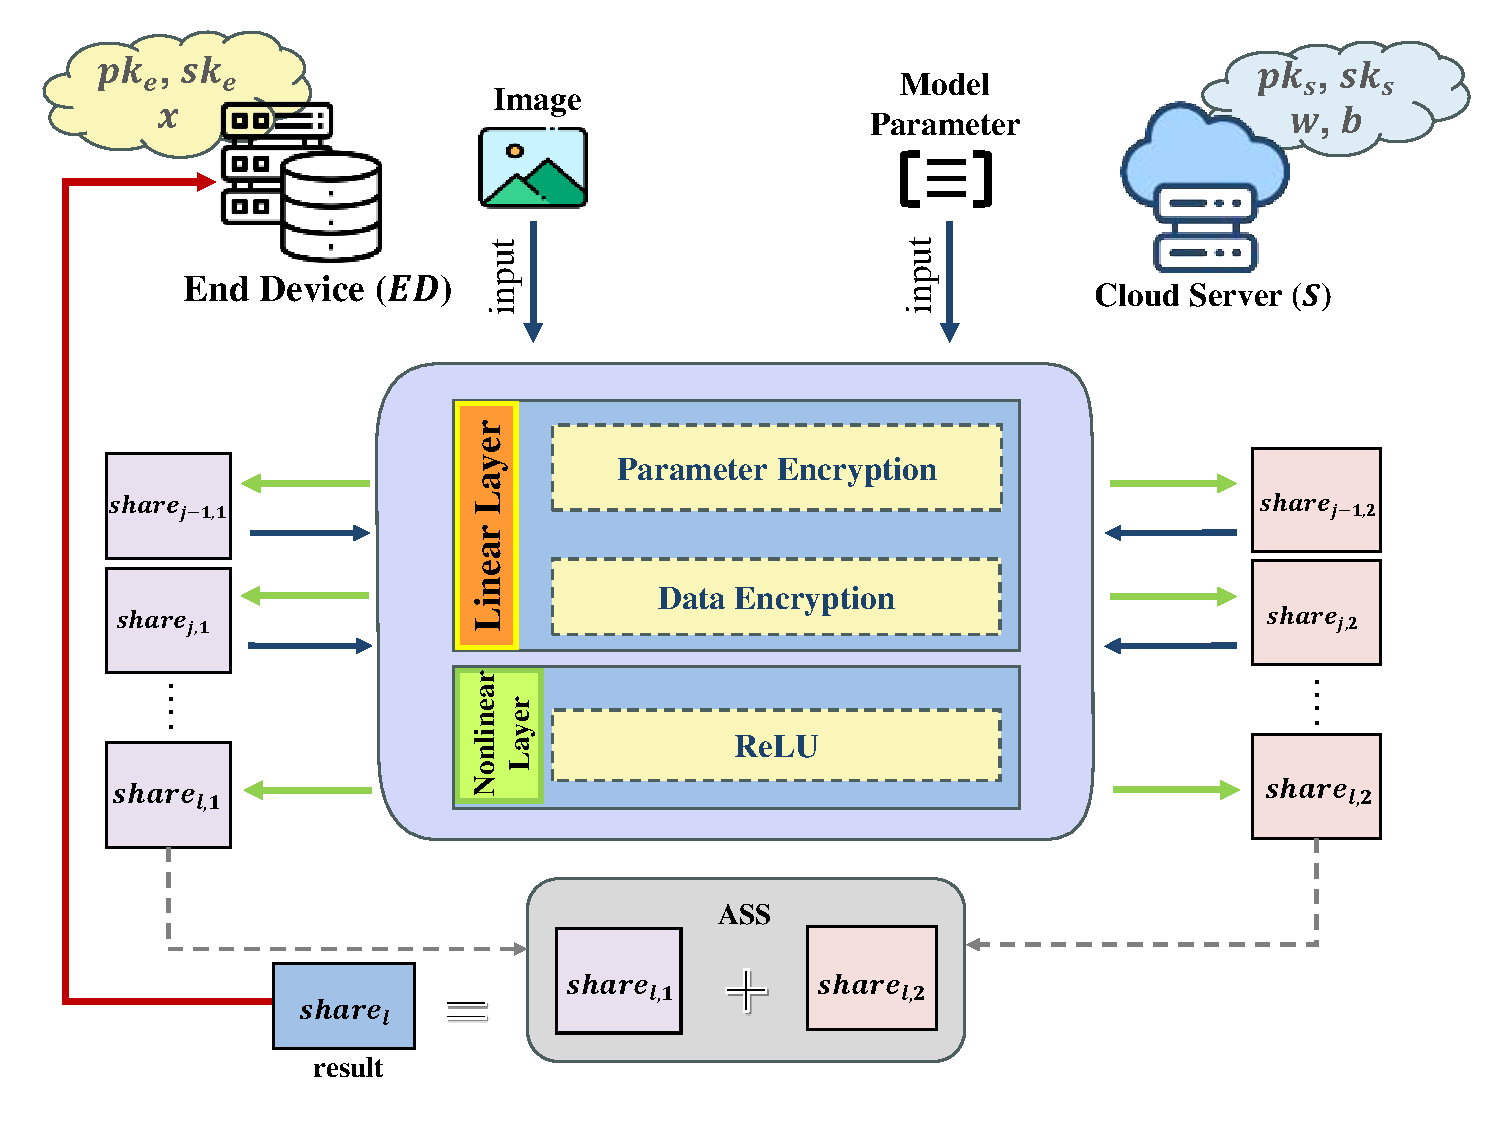
\includegraphics[width=1\linewidth]{fig1.pdf}
\caption{System model} \label{fig:system_model}
\end{figure}

Person: Persons are the people who input the image to the $ED$. 

$ED$: $ED$ receives the image sent by the user and extracts its features locally. These features are then split using additive secret sharing, with one part stored locally and the other sent to the cloud server. Finally, $ED$ combines the results from the cloud and local computations to produce the inference outcome.

$S$: $S$ is an auxiliary computational cloud server that receives the feature data sent by $ED$ after secret sharing. $S$ performs the necessary computations on the received data and then sends the computed results back to $ED$. 
 
%  TODO: 下面这段话应该放到后面
%  This architecture ensures both security and efficiency in face recognition processes by distributing computational tasks and securely handling sensitive data. Moreover, it leverages advanced cryptographic techniques to protect data privacy throughout the entire workflow.	

\subsection{Threat Model and Security Goal}
In our system, the main threats include: attackers intercepting and tampering with image data, feature data, or computation results transmitted between the $ED$ and $S$, leading to unauthorized access or data manipulation; the cloud server, or a compromised part of it, analyzing shared data to infer the original image or its features, thereby violating user privacy; and attackers targeting the $ED$ or cloud server to gain access to raw or secretly shared data, compromising the security of the entire system. Based on the above threat model, our security goals are listed as follows:
\begin{itemize}
     \item \textit{Data integrity and confidentiality}: Additive secret sharing to split the vectors into parts (e.g., $\langle x \rangle_1$ and $\langle x \rangle_2$) before uploading them to $S$. This ensures that no single server holds enough information to reconstruct the original data. Protect the image and its features from being exposed to unauthorized parties during transmission and at rest. Ensure that the data transmitted between $ED$ and the $S$ is not tampered with. 
     \item \textit{Collusion Resistance}: Ensure that only authorized entities $ED$ and $S$ can access and process encrypted feature vectors, preventing unauthorized inference of biometric information. If one of the servers is compromised or colludes with an attacker, they cannot reconstruct the original feature vectors without the shares from the other server.
 \end{itemize}
 
\section{MIND Design}
In this section, we first describe how images are shared using additive secret sharing at the $ED$, then detail the hierarchical cryptographic inference model, and finally illustrate the overall inference process. The notations utilized in this work are summarized in Table \ref{table:notations}.
% \subsection{Scheme Construction}
% 详细解释系统如何实现加法秘密共享和同态加密,包括技术细节和算法。

\subsection{Secret sharing of image features}
% In MIND, multiple organizations collaborate on tasks related to model training and data interaction. The data owned by these organizations are temporary and cannot be directly shared. It is assumed that all institutions involved in the training process are rigorously verified as non-malicious participants, ensuring they do not engage in activities such as poisoning attacks that could compromise the model or the training process.

As shown in Fig. \ref{fig:system_model}, $ED$ plays a dual role in this system. It is both a data receiver and a sender. As an end device, $ED$ first collects images. It then uses a local feature extraction model to extract image feature information. Fig. \ref{fig:ED_Models} shows the detailed data processing flow. To ensure data security, $ED$ uses additive secret sharing to securely split the feature information. After collecting an image, $ED$ first generates an n-dimensional random vector $\langle x \rangle_1$, with each element randomly selected from $\mathbb{Z}_t$. It then creates a second share, $\langle x \rangle_2$, by subtracting this random vector $\langle x \rangle_1$ from the original image vector $v$. This process is represented by the following formula:
$\langle x \rangle_2 = v - \langle x \rangle_1$
The sum of share $\langle x \rangle_1$ and share $\langle x \rangle_2$ equals the original image vector $v$. This design protects the privacy of feature information. It also enables secure distributed storage. Even when data is split and stored in a distributed manner, it can be securely reconstructed. This mechanism greatly enhances the system's security and privacy protection. At the same time, it maintains data usability and integrity.

\begin{figure}[ht]
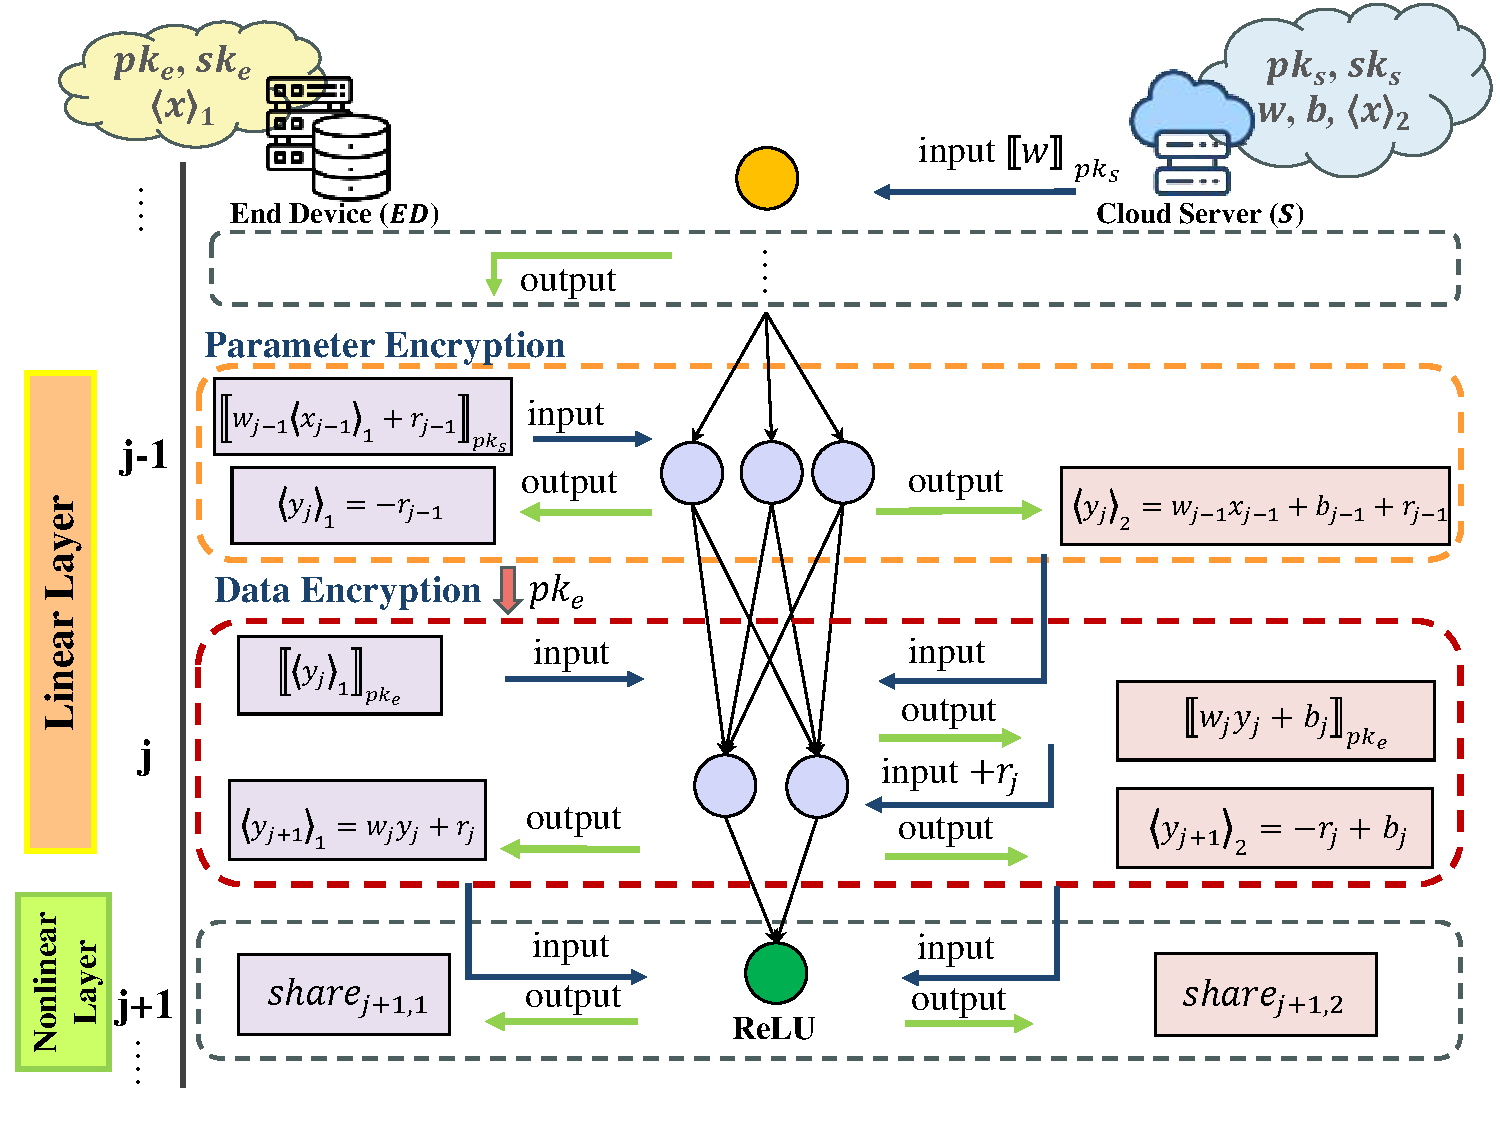
\includegraphics[width=1\linewidth]{fig2.pdf}
\caption{ED Secret Sharing Model} \label{fig:ED_Models}
\end{figure}

% In MIND, multiple institutions jointly perform tasks related to model training and data interaction.

% \subsection{Server homomorphic encryption}
%  The traditional method for encrypting the model training process between cloud servers involves directly encrypting the image data. Our research found that encrypting parameters in certain neural network layers, such as convolutional layers, can improve computational efficiency and reduce communication overhead without compromising model accuracy. We propose two encryption methods: data encryption and parameter encryption. By alternating between these two encryption methods during model training, we can effectively enhance the efficiency of the training process and reduce communication overhead. These methods are detailed below.

 \subsection{Parameter and Data Encryption}
Traditional encryption methods for collaborative inference between cloud servers and end devices often encrypt image data directly. While this approach protects data privacy, it has limitations in terms of computational efficiency and communication overhead. To address these issues, we propose MIND, a novel eNd-clouD collaborative encryption method. This new approach divides the encryption process into two parts: Model parameter encryption, Image data encryption. Our method applies these two encryption techniques to different network layers. This division allows for a more efficient and flexible approach to data protection.

As described in \PEnc~(Algorithm \ref{alg:Parameter}), $S$ encrypts the model weights $w_p$ using public key $pk_s$ and transmitting the encrypted weights $\llbracket w \rrbracket_{pk_s}$ to $ED$. Upon receiving $\llbracket w_p \rrbracket_{pk_s}$, $ED$ performs a homomorphic multiplication operation to evaluate the product of $\llbracket w_p \rrbracket_{pk_s}$ and $\langle x \rangle_1$, yielding the result $\llbracket w_p \langle x \rangle_1\rrbracket_{pk_s} = \llbracket w_p \times \langle x \rangle_1 \rrbracket_{pk_s}$. Subsequently, $ED$ introduces a random number $r_1\in \mathbb{Z}_t$ and calculates the encrypted result $\llbracket C \rrbracket_{pk_s}=\llbracket w_p \langle x \rangle_1 + r_1 \rrbracket_{pk_s}$, which is then sent back to $S$. $S$ decrypts $\llbracket C \rrbracket_{pk_s}$ to retrieve the value $w_p\langle x \rangle_1+r_1$. Next, $S$ calculates the result $\langle y_p\rangle_2= w_p(\langle x \rangle_1 + \langle x \rangle_2)+r_1+b=w_px+r_1+b$, $ED$ obtains the result $\langle y_p\rangle_1=-r_1$. 
\begin{algorithm}[htbp]
	\caption{\PEnc($\langle x \rangle_1,\langle x \rangle_2,w,b) \rightarrow (\langle y_p\rangle_1, \langle y_p\rangle_2$)}
    \label{alg:Parameter}
    \LinesNumbered
	\KwIn{$ED$ holds $\langle x \rangle_1$. \\
	\hspace{33pt}$S$ holds $\langle x \rangle_2$, $w$, and $b$.}
    \KwOut {Secret shares $\langle y_p \rangle_1 $ and $\langle y_p \rangle_2$.}
     $S$ sends $\llbracket w_p\rrbracket_{pk_s}$ to $ED$;
    
     $ED$ evaluates $\llbracket w_p\langle x \rangle_1 \rrbracket_{pk_s} = \llbracket w_p \rrbracket_{pk_s} \otimes \llbracket \langle x \rangle_1 \rrbracket_{pk_s}$;
    
     $ED$  calculates $\llbracket C\rrbracket_{pk_s} = \llbracket w_p\langle x \rangle_1 \rrbracket_{pk_s} \oplus \llbracket r_1 \rrbracket_{pk_s}$;
     
     $ED$ sends $\llbracket C\rrbracket_{pk_s}$ back to $S$;
    
     $S$ decrypts $\llbracket C\rrbracket_{pk_s}$ to get $w_p\langle x \rangle_1 + r_1$;
     
     $ED$ obtains $\langle y_p\rangle_1=-r_1$ and $S$ obtains $\langle y_p\rangle_2 = w_p x  + b_1 + r_1$.
\end{algorithm}

As illustrated in \DEnc~(Algorithm \ref{alg:DataHE}), $ED$ encrypts its secret share $\langle y_p \rangle_1$ of the held data using the public key $pk_e$ and transmits $\llbracket\langle y_p \rangle_1\rrbracket_{pk_e}$ to server $S$ for model inference. Upon receiving the encrypted secret share, $S$ performs a homomorphic addition operation to combine the two encrypted portions of the secret share, $\llbracket\langle y_p \rangle_1\rrbracket_{pk_e}$ and $\llbracket\langle y_p \rangle_2\rrbracket_{pk_e}$, into a single encrypted value $\llbracket y_p \rrbracket_{pk_e}=\llbracket \langle y_p \rangle_1 +  \langle y_p \rangle_2\rrbracket_{pk_e}$. After that, $S$ performs homomorphic multiplication between the $\llbracket y_p \rrbracket_{pk_e}$ and the model weights $w_d$ as $\llbracket y_p\times w_d \rrbracket_{pk_e}$. Simultaneously, a random number $r_2 \in \mathbb{Z}_t$ is generated and summed with the result. This step ensures that the data remains encrypted throughout the computation process, maintaining data privacy and security during inference.
 
After $S$ completes the homomorphic encryption operations, it sends its computed share back to $ED$. At this point, both servers possess partial results, $\langle y_d \rangle_1$ and $\langle y_d \rangle_2$, which are the respective secret shares. These secret shares are then combined through a secure protocol to reconstruct the complete result $y_d$.
\begin{algorithm}[htbp]
	\caption{DEnc($\langle y_p \rangle_1,\langle y_p \rangle_2,w,b) \rightarrow (\langle y_d\rangle_1,\langle y_d\rangle_2$)}
    \label{alg:DataHE}
    \LinesNumbered
	\KwIn{$ED$ holds $\langle y_p \rangle_1$.\\
	\hspace{32pt}$S$ holds $\langle y_p \rangle_2, w$, and $b$.}
    \KwOut{Secret shares $\langle y_d \rangle_1 $ and $\langle y_d \rangle_2$.}
    $ED$ sends $\llbracket\langle y_p \rangle_1\rrbracket_{pk_e}$ to $S$;
    
    $S$ evaluates $\llbracket\langle y_p \rangle_1\rrbracket_{pk_e} = \llbracket \langle y_p \rangle_1 \rrbracket_{pk_e}  \oplus  \llbracket\langle y_p\rangle_2\rrbracket_{pk_e}$;
    
    $S$ computes $\llbracket w_d \times y_p \rrbracket_{pk_e} = \llbracket w_d \rrbracket_{pk_e} \otimes \llbracket  y_p \rrbracket_{pk_e}$;
    
    $S$ calculates $\llbracket C \rrbracket_{pk_e} = \llbracket w_d \times y_p \rrbracket_{pk_e} \oplus \llbracket r_2 \rrbracket_{pk_e}$;
    
    $S$ returns $\llbracket C \rrbracket_{pk_e}$ to $ED$;
    
    $ED$ obtains $\langle y_d\rangle_1=w_d \times y_p+r_2$ and $S$ obtains $\langle y_d \rangle_2 = w_d \times y_p-r_2+b_2$.
\end{algorithm}

This approach not only preserves the confidentiality of the input data but also allows for secure computations on encrypted data, enabling privacy-preserving machine learning in cloud environments. The use of homomorphic encryption techniques in this manner facilitates collaborative model training and inference without exposing sensitive information to potential security threats.


% While experimenting we found that the computational consumption of different layers in a neural network varies significantly. Typically, the number of parameters in the convolutional layer is less than the amount of data, while the number of parameters in the linear layer is greater than the amount of data. However, if the batch size of the training is large, the number of parameters may be less than the amount of data. The number of parameters for the linear layer can be determined by defining a fully connected layer with a specified number of input features and output features. In this context, the number of parameters is calculated by multiplying the number of input features by the number of output features. The amount of input data is calculated by multiplying the number of input features by the batch size. To ensure optimal performance, the batch size needs to be larger than the output features.


% Then $ED$ and $S$ are safely combined to reconstruct the complete result $y=wx+b$.

\subsection{Inference Overview}

\begin{algorithm}[htbp]
	\caption{The Search Procedure}
	\label{algo:search}
	\LinesNumbered
	\KwIn{
	$ED$ holds an image $x$ and batchsize $B$.
	Server $S$ holds the network model $M = M_1 || M_2 \dots || M_n$.
	The weights and biases of each layer $M_j$ are $w_j$ and $b_j$, respectively.
	Define $k$ as the number of model cut layers
	}
	\KwOut{
	
	}
    $ED$ sets $\langle x_0 \rangle_1=x$ and  $S$ sets the $\langle x_0 \rangle_2 = 0$.
    
    % $S$ sends $\llbracket w \rrbracket_{pk_s}$ to $ED$.

	\For{$j=1$ to $n$}{
	    \eIf{$ j \leq k$}{
	            ($\langle x_{j} \rangle_1$, $\langle x_{j} \rangle_2 ) \leftarrow$ $\PEnc(\langle x_{j - 1}\rangle_1,\langle x_{j-1}\rangle_2,w_j,b_j$);
	        }{
	             ($\langle x_{j} \rangle_1$, $\langle x_{j} \rangle_2 ) \leftarrow$ $\DEnc(\langle x_{j - 1}\rangle_1,\langle x_{j-1}\rangle_2,w_j,b_j$);
	            
	           % $ED$ and $S$ call \DEnc~$(\langle y_{p_j} \rangle_1,\langle y_{p_j} \rangle_2,w_j,b_j \rightarrow \langle y_{d_j}\rangle_1, \langle y_{d_j}\rangle_2)$ to get $\langle y_{d} \rangle_1$ and $\langle y_{d} \rangle_2$, respectively;
	        }
	}
    
    $ED$ defines $\langle y \rangle_1=\langle x_n \rangle_1$ and  $S$ defines the $\langle y \rangle_2=\langle x_n \rangle_2$.
    
   $S$ sends $\langle y \rangle_2$ to $ED$.
    
    $ED$ reconstructs the final inference result by computing $y = \langle y \rangle_1 + \langle y \rangle_2$.
\end{algorithm}

\begin{figure*}[ht]
\centering
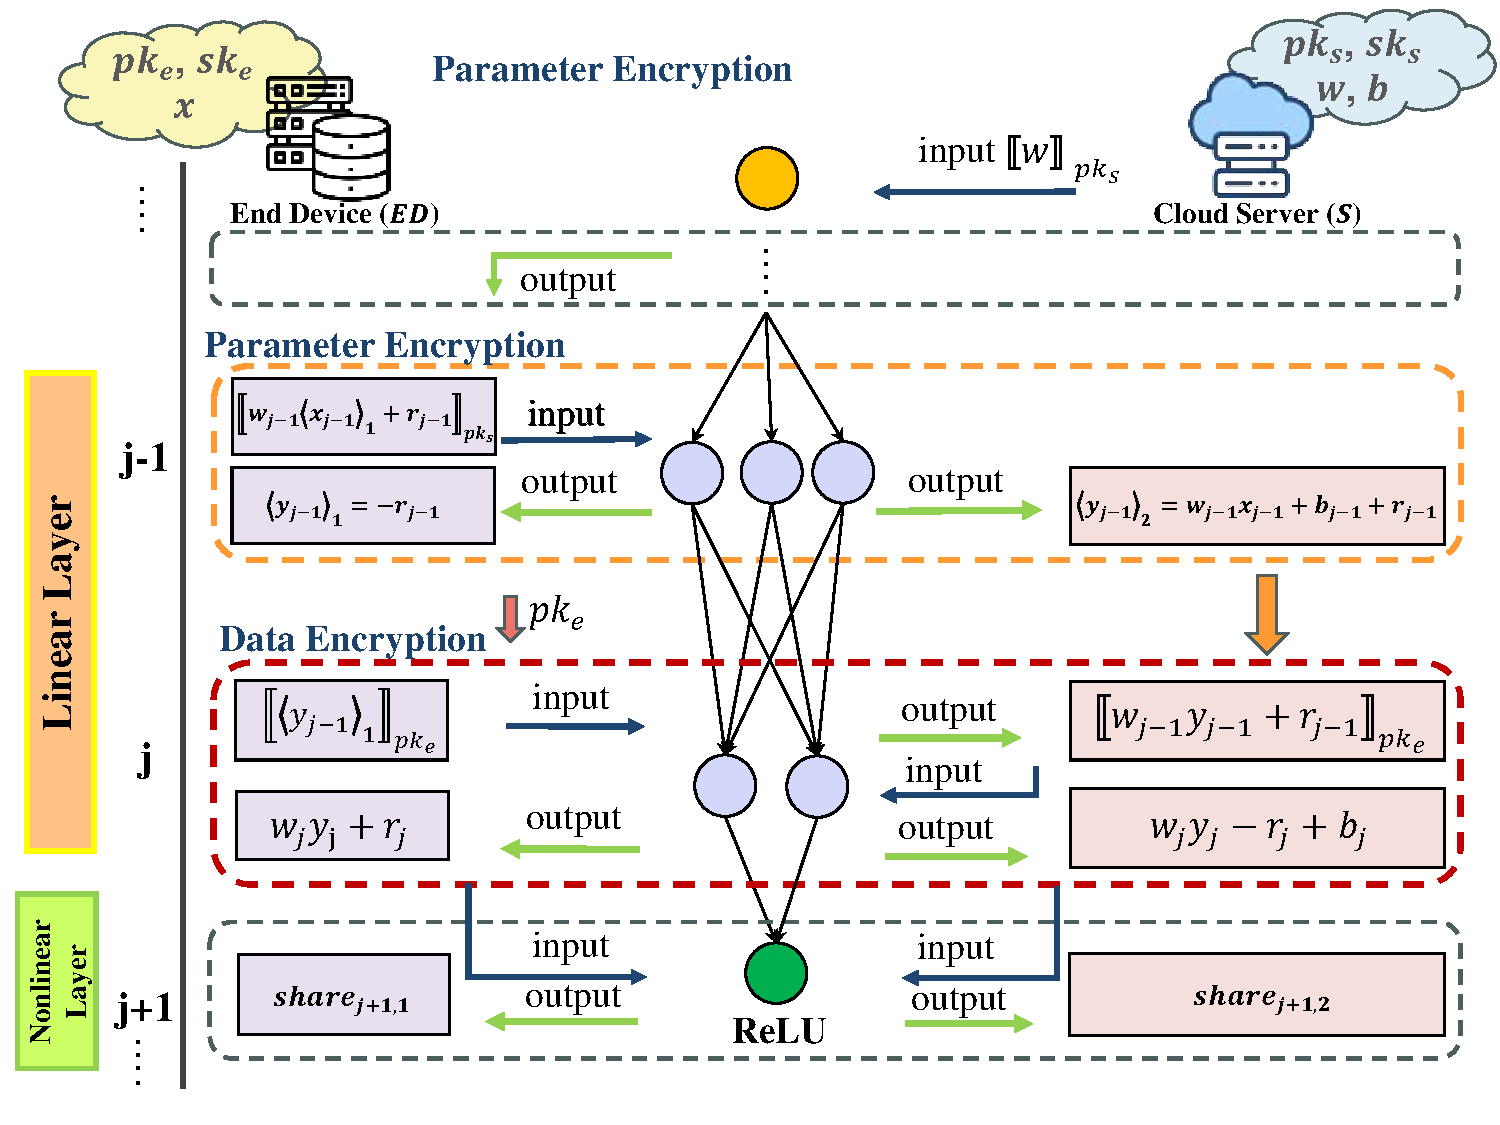
\includegraphics[scale=0.6]{fig3.pdf}
\caption{Serve Models} \label{fig:Serve_Models}
\end{figure*}
In this inference process, assume $ED$ holds an image $img$ with the size $n\times m$. $S$ is the main computational cloud server where the model $M$ is stored. The overall model $M$ is composed of multiple sub-models $M=M_1 || M_2 \dots M_n$. Each layer of the model $M_j$ is associated with specific weights $w_{j}$ and biases $b_{j}$ for $j \in \{1, 2, \dots, n\}$.
Formally, model $M$ can be represented as a collection of layer-specific parameters $M=\{(w_{1},b_{1}),(w_{2},b_{2}),\dots,(w_{n},b_{n})\}$, where $n$ denotes the number of layers in $M$.

The computation at each layer is denoted as $x_j = f_j(x_{j-1})$, where $j$ denotes the current network layer and $x_j=\langle x_j \rangle_1 + \langle x_j \rangle_2$. All intermediate outputs of each layer are secretly shared between $ED$ and $S$, except for the final output $y$. At the beginning, we keep the secret sharing form for all layers $f_j$. Here, $f_j$ represents a secure computation protocol running on secret sharing. The protocol obtains the secret share $\langle x_{j-1} \rangle_i$ of the previous layer's output from both parties and generates the secret share $\langle x_j \rangle_i$ of the current layer. This can be expressed as:
\begin{equation}
    \langle x_j \rangle_1+\langle x_j \rangle_2 = f_j(\langle x_{j-1} \rangle_1 + \langle x_{j-1} \rangle_2).
\end{equation}

The process begins with the server $S$ encrypting a subset of the model parameters $w_j$ for $j \in [1,k]$ and transmitting these encrypted parameters $\llbracket w_j \rrbracket_{pk_s}$ to $ED$. Upon receiving the encrypted parameters , the $ED$ uses homomorphic encryption to perform inference on the initial layers of the model. The $ED$ then encrypts the resulting intermediate results and sends them to $S$. Subsequently, $S$ continues the inference on the remaining layers of the model using the encrypted data provided by the $ED$. This process ensures that both the sensitive parameters and image data are protected through encryption before further processing or transmission.

% as shown in Fig. \ref{fig:ED_Models} and \ref{fig:Serve_Models}, $ED$ separates the original image feature vector $x$ using an additive secret sharing scheme. 
Specifically, as described in Algorithm \ref{algo:search}, the initial input is $x_0=x$ split between  $ED$ and $S$, with $ED$ setting $\langle x_0\rangle_1=x$ and $S$ setting the $\langle x_0\rangle_2=0$. 

For each layer $j$ from 1 to $n$, if $j \leq k$ (where $k$ is the number of layers processed by the $ED$), the $ED$ and $S$ use the \PEnc~method to compute the encrypted shares $\langle x_j \rangle_1$ and $\langle x_j \rangle_2$. Otherwise, we use \DEnc~method.
 After all layers are processed, $ED$ holds $\langle y \rangle_1=\langle x_n\rangle_1$ and $S$ holds $\langle y \rangle_2=\langle x_n\rangle_2$. Finally, $S$ then sends $\langle y \rangle_2$ to $ED$, which then reconstructs the final inference result by computing $y=\langle y \rangle_1+\langle y \rangle_2$.

In summary, this algorithm ensures that the computational process is carried out securely and efficiently, with each server only having access to a share of the data. By employing secret sharing and encryption techniques, the privacy of the input image is preserved throughout the inference procedure, thereby providing a robust solution for secure cloud-based neural network computations.
%In forward propagation, $ED$ draws a batch of input data $\langle x_0\rangle_1$ to feed into the model $M_1$.  


% The overall model $m$ is composed of multiple sub-models $m=\{m_1,m_2,\dots,m_n\}$. Each sub-model $m_i$ consists of several layers, and for each layer $j$ in the sub-model $m_i$, there are associated weights $w_{ij}$ and biases $b_{ij}$. 
% Formally, each sub-model $m_i$ can be represented as a collection of layer-specific parameters $m_i=\{(w_{i1},b_{i1}),(w_{i2},b_{i2}),\dots,(w_{ik},b_{ik})\}$, where $k_i$ denotes the number of layers in $m_i$. Therefore, the overall model m can be expressed as $m =\{(w_{i1}, b_{i1}), (w_{i2}, b_{i2}), \dots,$ $(w_{ik_i}, b_{ik_i}) | i=1,2,\dots,n\}$, with each $m_i$ containing its corresponding set of weights and biases for each layer.

\section{Experiment and Result}
In the MIND experiments, we conduct comparison studies, evaluating the layered encryption method against the encryption method proposed in this paper. The evaluation criteria include accuracy, F1 score, recall, runtime, and communication cost.

\subsection{Setting}
\subsubsection{Environment.} Our solution is implemented in python, and the experiments run on two servers that both equipped with an AMD EPYC 7402 CPU and 128 GB of RAM.
\subsubsection{Dataset.} 
We employ the widely-used MNIST datasets \cite{xiao2017fashion} to train and evaluate our models. To ensure the data is suitable for model input, the following preprocessing steps are applied. The MNIST dataset comprises 60,000 training images and 10,000 test images, each a 28$\times$28 pixel grayscale image of handwritten digits. We normalize the pixel values to the [0, 1] range and implemented data augmentation techniques such as random rotations and translations during training. The CIFAR-10 dataset consists of 50,000 training images and 10,000 test images, each a 32$\times$32 pixel color image categorized into 10 classes. We standardize the images so that the pixel values for each channel have zero mean and unit variance. We trained each image neural network using the training dataset for 10 epochs. Additionally, we employ data augmentation techniques, including random cropping, horizontal flipping, and color jittering, to enhance the model's generalization capability.




\subsubsection{Parameters.} 
The learning rate $\eta$ is set to 0.01 to accelerate model convergence while maintaining stability. For the MNIST dataset, a batch size $B$ of 32 is used, while a batch size $B$ of 64 is employed for the CIFAR-10 dataset. The momentum $\gamma$ is configured at 0.8 to effectively smooth the update process and reduce gradient oscillations during training. Additionally, the gradient bound estimation $C$ is set to 8 to limit the maximum gradient value and prevent gradient explosion.

\subsection{Effectiveness}
In this subsection, we evaluate the effectiveness of the scheme. The MIND scheme we propose employs hierarchical encryption, whereas the non-hierarchical encryption scheme is referred to as the Naive scheme. We achieve this by utilizing models with different architectures on the MNIST dataset, specifically mnist aby3, mnist sphinx, mnist quotient 3$\times$128, and mnist quotient 2$\times$512. We compare the Accuracy, Precision, Recall, and F1 Score between hierarchical encryption schemes and non-hierarchical encryption schemes based on these MNIST models.

\begin{table*}[ht]
\centering
\caption{Feasibility Evaluation}
\label{tab:effectiveness}
\begin{tabular}{lcccccc}
\toprule[1pt]
Model & Schemes & Accuracy & Precision & Recall & F1 Score  \\
\midrule[1pt]
\multirow{2}{*}{mnist aby3} & Naive & 0.978 & 0.978 & 0.978 & 0.978  \\
                            & MIND & 0.978 & 0.978 & 0.978 & 0.978  \\ \cline{1-6}
\multirow{2}{*}{mnist sphinx} & Naive & 0.991 & 0.991 & 0.990 & 0.991  \\
                            & MIND & 0.991 & 0.991 & 0.990 & 0.991  \\ \cline{1-6}
\multirow{2}{*}{mnist quotient 3$\times$128} & Naive & 0.978 & 0.978 & 0.978 & 0.978  \\
                            & MIND & 0.978 & 0.978 & 0.978 & 0.978  \\ \cline{1-6}
\multirow{2}{*}{mnist quotient 2$\times$512} & Naive & 0.980 & 0.980 & 0.980 & 0.980  \\
                            & MIND & 0.980 & 0.980 & 0.980 & 0.980  \\
\bottomrule[1pt]
\end{tabular}
\vspace{-6pt}
\begin{flushleft}
\begin{adjustwidth}{90pt}{70pt}  % 这里调整Note与左右边界的距离
\textbf{Note.}
$\text{Accuracy} = \frac{\text{TP} + \text{TN}}{\text{TP} + \text{TN} + \text{FP} + \text{FP}}$,
$\text{Precision} = \frac{\text{TP}}{\text{TP} + \text{FP}}$,
$\text{Recall} = \frac{\text{TP}}{\text{TP} + \text{FP}}$,
$\text{F1 Score} = 2 \times \frac{\text{Precision} \times \text{Recall}}{\text{Precision} + \text{Recall}}$ 
(TP: True Positive, TN: True Negative, FP: False Positive, FN: False Negative).
\end{adjustwidth}
\end{flushleft}
\end{table*}

According to the results shown in Table \ref{tab:effectiveness}, we can observe that there is no difference in the recognition accuracy between the hierarchical encryption scheme and the non-hierarchical encryption scheme. Therefore, we can conclude that there is no significant difference between hierarchical encryption and non-hierarchical encryption when performing facial recognition. This indicates that MIND is a feasible and effective privacy protection scheme for facial recognition.

\subsection{Efficiency}
To demonstrate that MIND can reduce both runtime and communication cost, we evaluated and compared the hierarchical encryption scheme of MIND with the Naive scheme in terms of runtime and communication cost. As illustrated in Figure \ref{fig:efficiency}, we can observe that for the four MNIST models: mnist aby3, mnist sphinx, mnist quotient 3$\times$128, and mnist quotient 2$\times$512, the transmission required by the MIND scheme is consistently lower than that of the Naive scheme. This reduction is attributed to the efficiency gains achieved through the hierarchical encryption, which effectively enhances performance and consequently lowers the runtime of MIND.

According to Figure \ref{subfig:aby3}, it can be observed that the MIND scheme is most effective in reducing communication cost when applied to the mnist aby3 model and is most effective in reducing runtime when applied to the mnist quotient 2x512 model. In our experiments, using the Naive encryption scheme required a communication cost of 1933MB, whereas the MIND scheme only required 1008MB, resulting in a reduction of approximately 49.42\% in communication cost, and The MIND scheme reduced the runtime by approximately 10.34\% compared to the Naive scheme. 

\begin{figure}[ht]
    \centering
    \subfigure[mnist aby3]{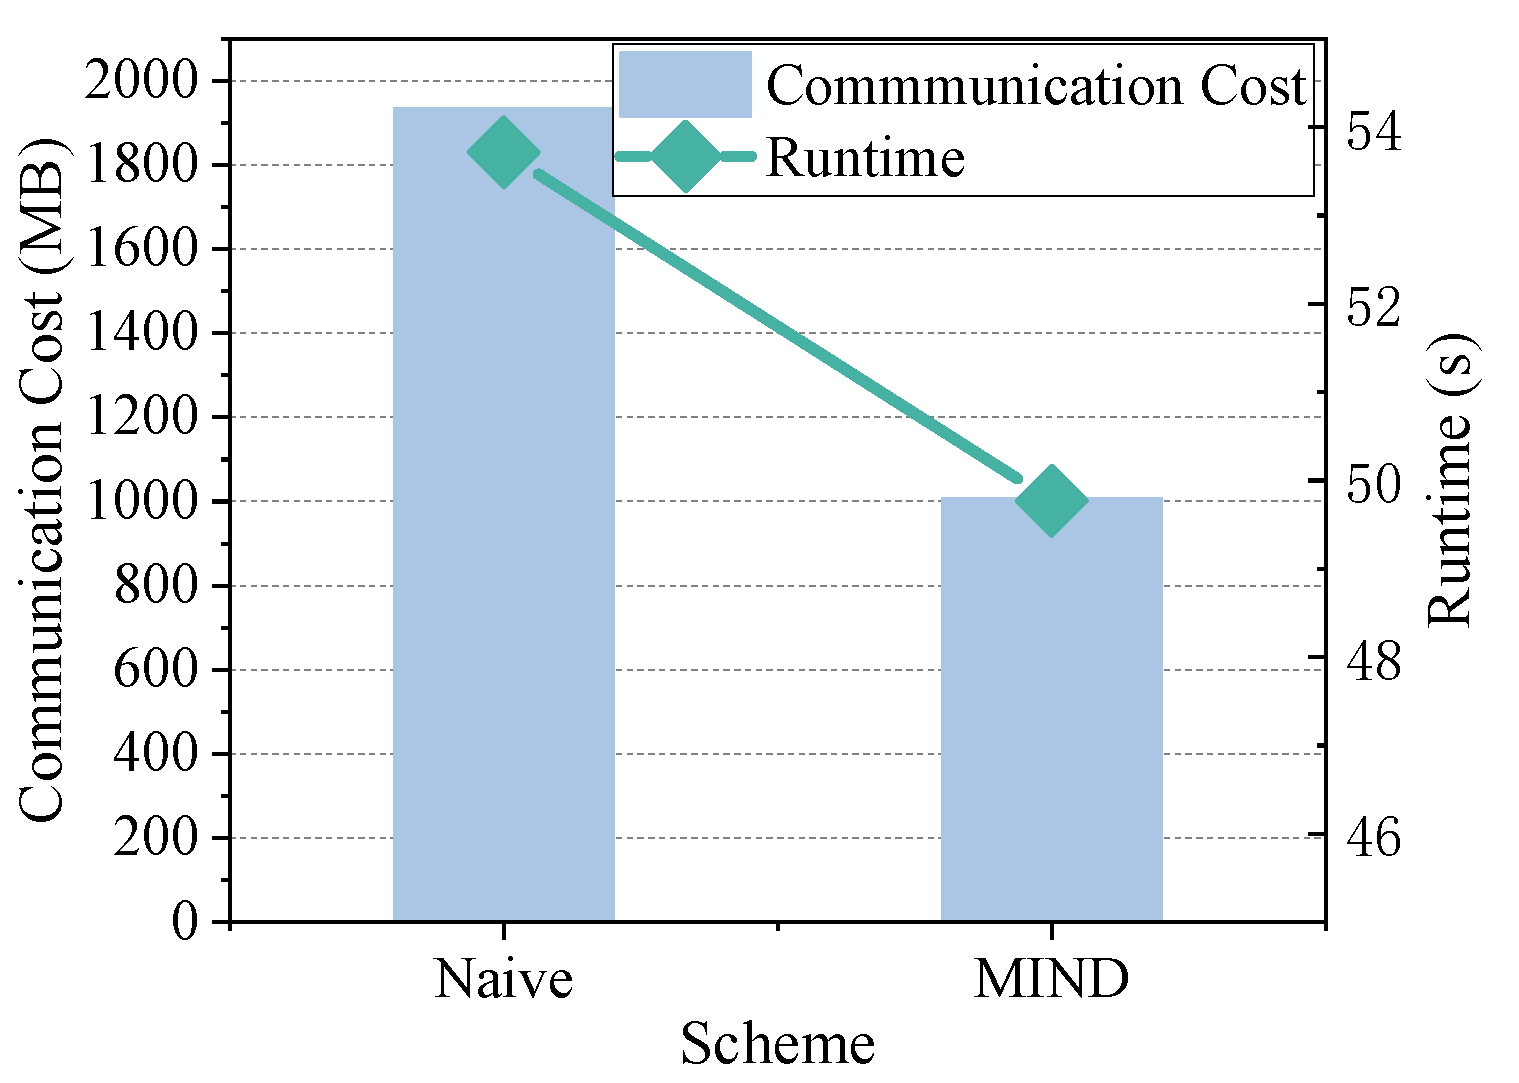
\includegraphics[width=.45\columnwidth]{exp/minst_aby3.pdf}\label{subfig:aby3}} \hspace{5pt}
    \subfigure[mnist sphinx]{\includegraphics[width=.45\columnwidth]{exp/spinx.pdf}\label{subfig:sphinx}} \\
    \subfigure[mnist quotient 3$\times$128]{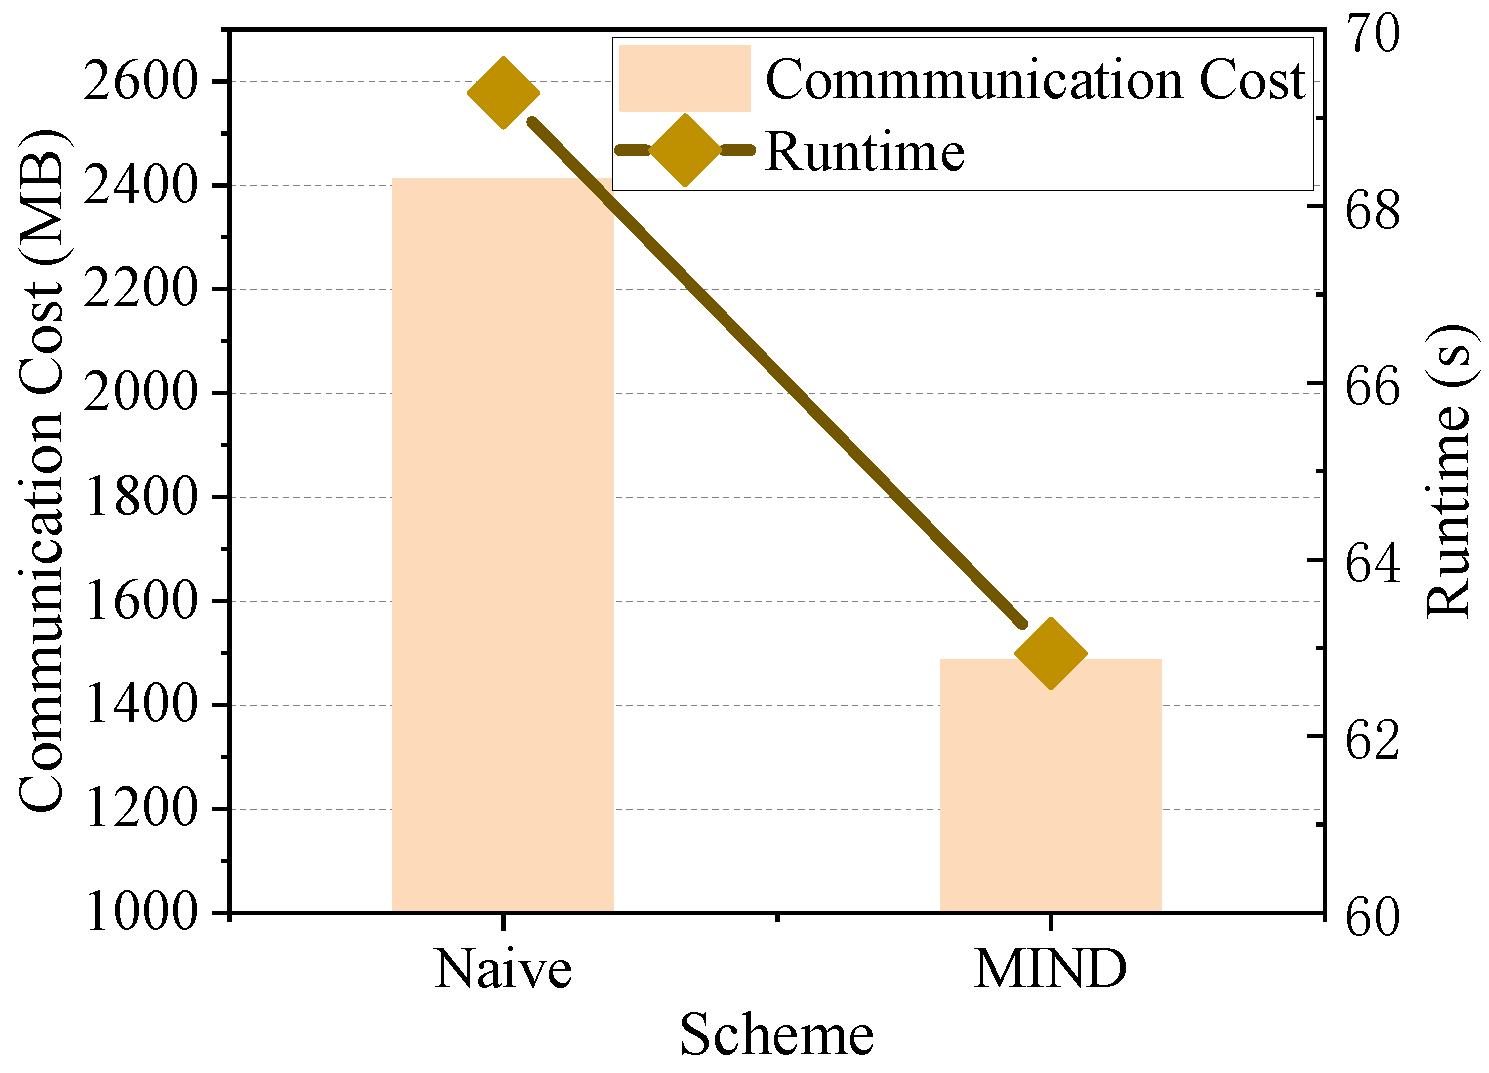
\includegraphics[width=.45\columnwidth]{exp/quotient_3.pdf}\label{subfig:quotient_3x128}} \hspace{5pt}
    \subfigure[mnist quotient 2$\times$512]{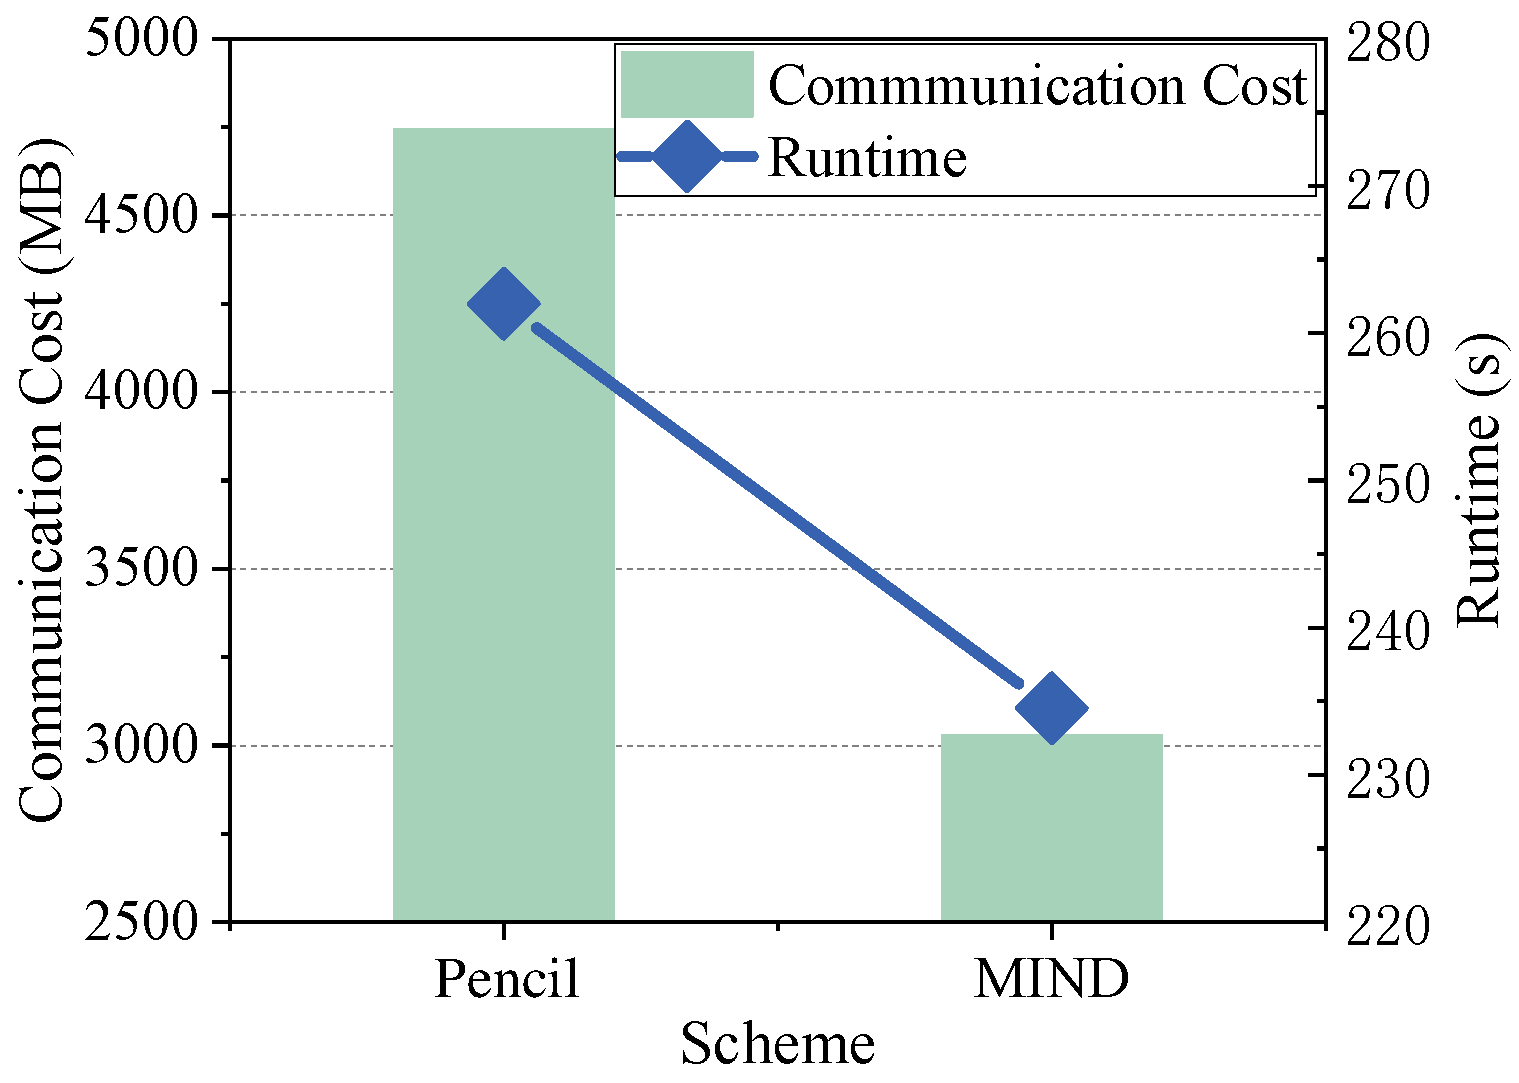
\includegraphics[width=.46\columnwidth]{exp/quotient_2.pdf}\label{subfig:quotient_2x512}}
    \caption{Efficiency evaluation.}
    \label{fig:efficiency}
\end{figure}

% \begin{figure}[ht]
% \centering
% 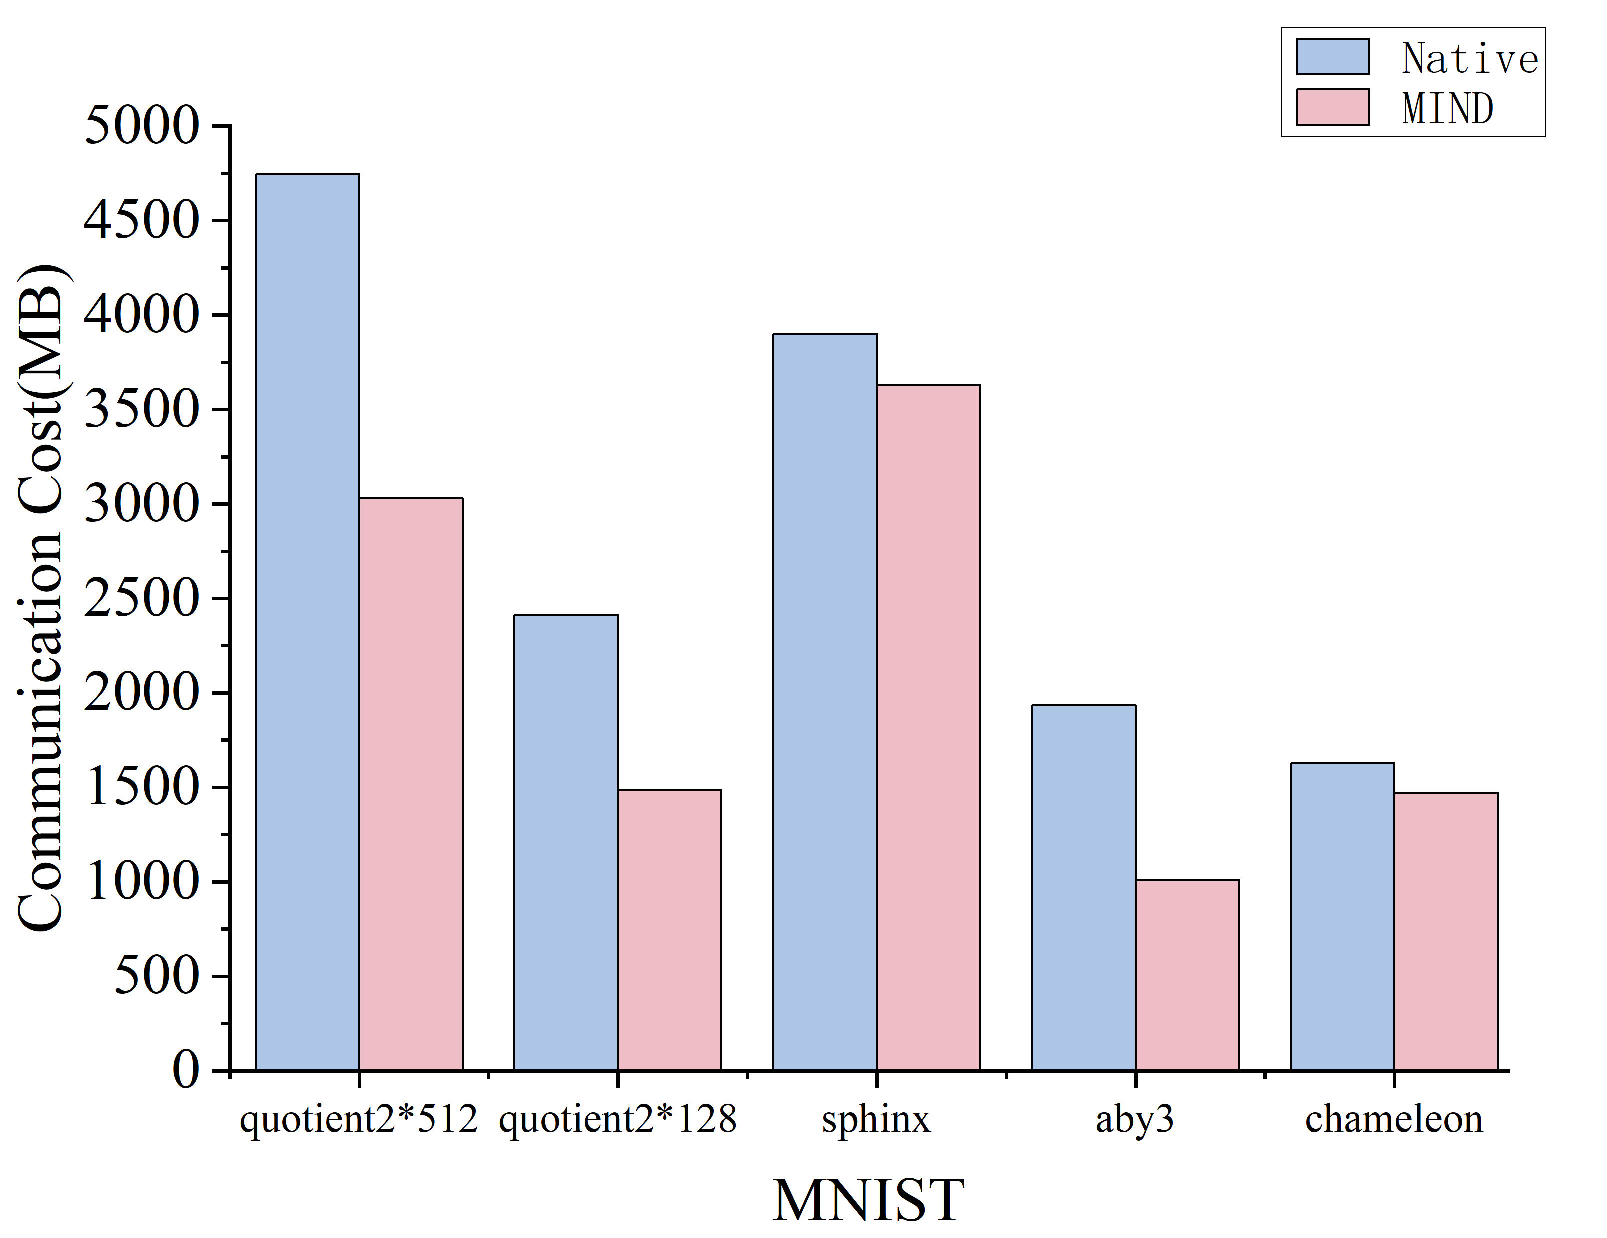
\includegraphics[width=1\linewidth]{Communication_cost.pdf}
% \caption{Communication cost} \label{fig:cost}
% \end{figure}

\section{Conclusion}
In this paper, we introduce MIND, a privacy-preserving inference framework designed to address the privacy challenges associated with the task of collaborative inference computation in the end-cloud. MIND utilizes advanced encryption techniques, including secret sharing and homomorphic encryption, to secure data and model parameters throughout the cloud inference process. Within the MIND framework, we design a layered encryption scheme that dynamically adapts encryption methods between the end device and cloud servers to significantly reduce computation and communication overheads.

Our experimental results show that this innovative solution not only greatly enhances data protection but also effectively ensures that the performance of the inference model remains unaffected. As a result, MIND provides robust privacy protection without compromising operational efficiency, establishing itself as a secure and efficient cloud-based collaborative inference model with significant practical value and relevance.


% \subsection{Equations}
% Number equations consecutively. To make your 
% equations more compact, you may use the solidus (~/~), the exp function, or 
% appropriate exponents. Italicize Roman symbols for quantities and variables, 
% but not Greek symbols. Use a long dash rather than a hyphen for a minus 
% sign. Punctuate equations with commas or periods when they are part of a 
% sentence, as in:
% \begin{equation}
% a+b=\gamma\label{eq}
% \end{equation}

% Be sure that the 
% symbols in your equation have been defined before or immediately following 
% the equation. Use ``\eqref{eq}'', not ``Eq.~\eqref{eq}'' or ``equation \eqref{eq}'', except at 
% the beginning of a sentence: ``Equation \eqref{eq} is . . .''

% \subsection{\LaTeX-Specific Advice}

% Please use ``soft'' (e.g., \verb|\eqref{Eq}|) cross references instead
% of ``hard'' references (e.g., \verb|(1)|). That will make it possible
% to combine sections, add equations, or change the order of figures or
% citations without having to go through the file line by line.

% Please don't use the \verb|{eqnarray}| equation environment. Use
% \verb|{align}| or \verb|{IEEEeqnarray}| instead. The \verb|{eqnarray}|
% environment leaves unsightly spaces around relation symbols.

% Please note that the \verb|{subequations}| environment in {\LaTeX}
% will increment the main equation counter even when there are no
% equation numbers displayed. If you forget that, you might write an
% article in which the equation numbers skip from (17) to (20), causing
% the copy editors to wonder if you've discovered a new method of
% counting.

% {\BibTeX} does not work by magic. It doesn't get the bibliographic
% data from thin air but from .bib files. If you use {\BibTeX} to produce a
% bibliography you must send the .bib files. 

% {\LaTeX} can't read your mind. If you assign the same label to a
% subsubsection and a table, you might find that Table I has been cross
% referenced as Table IV-B3. 

% {\LaTeX} does not have precognitive abilities. If you put a
% \verb|\label| command before the command that updates the counter it's
% supposed to be using, the label will pick up the last counter to be
% cross referenced instead. In particular, a \verb|\label| command
% should not go before the caption of a figure or a table.

% Do not use \verb|\nonumber| inside the \verb|{array}| environment. It
% will not stop equation numbers inside \verb|{array}| (there won't be
% any anyway) and it might stop a wanted equation number in the
% surrounding equation.

% \subsection{Some Common Mistakes}\label{SCM}
% \begin{itemize}
% \item The word ``data'' is plural, not singular.
% \item The subscript for the permeability of vacuum $\mu_{0}$, and other common scientific constants, is zero with subscript formatting, not a lowercase letter ``o''.
% \item In American English, commas, semicolons, periods, question and exclamation marks are located within quotation marks only when a complete thought or name is cited, such as a title or full quotation. When quotation marks are used, instead of a bold or italic typeface, to highlight a word or phrase, punctuation should appear outside of the quotation marks. A parenthetical phrase or statement at the end of a sentence is punctuated outside of the closing parenthesis (like this). (A parenthetical sentence is punctuated within the parentheses.)
% \item A graph within a graph is an ``inset'', not an ``insert''. The word alternatively is preferred to the word ``alternately'' (unless you really mean something that alternates).
% \item Do not use the word ``essentially'' to mean ``approximately'' or ``effectively''.
% \item In your paper title, if the words ``that uses'' can accurately replace the word ``using'', capitalize the ``u''; if not, keep using lower-cased.
% \item Be aware of the different meanings of the homophones ``affect'' and ``effect'', ``complement'' and ``compliment'', ``discreet'' and ``discrete'', ``principal'' and ``principle''.
% \item Do not confuse ``imply'' and ``infer''.
% \item The prefix ``non'' is not a word; it should be joined to the word it modifies, usually without a hyphen.
% \item There is no period after the ``et'' in the Latin abbreviation ``et al.''.
% \item The abbreviation ``i.e.'' means ``that is'', and the abbreviation ``e.g.'' means ``for example''.
% \end{itemize}
% An excellent style manual for science writers is \cite{b7}.

% \subsection{Authors and Affiliations}\label{AAA}
% \textbf{The class file is designed for, but not limited to, six authors.} A 
% minimum of one author is required for all conference articles. Author names 
% should be listed starting from left to right and then moving down to the 
% next line. This is the author sequence that will be used in future citations 
% and by indexing services. Names should not be listed in columns nor group by 
% affiliation. Please keep your affiliations as succinct as possible (for 
% example, do not differentiate among departments of the same organization).

% \subsection{Identify the Headings}\label{ITH}
% Headings, or heads, are organizational devices that guide the reader through 
% your paper. There are two types: component heads and text heads.

% Component heads identify the different components of your paper and are not 
% topically subordinate to each other. Examples include Acknowledgments and 
% References and, for these, the correct style to use is ``Heading 5''. Use 
% ``figure caption'' for your Figure captions, and ``table head'' for your 
% table title. Run-in heads, such as ``Abstract'', will require you to apply a 
% style (in this case, italic) in addition to the style provided by the drop 
% down menu to differentiate the head from the text.

% Text heads organize the topics on a relational, hierarchical basis. For 
% example, the paper title is the primary text head because all subsequent 
% material relates and elaborates on this one topic. If there are two or more 
% sub-topics, the next level head (uppercase Roman numerals) should be used 
% and, conversely, if there are not at least two sub-topics, then no subheads 
% should be introduced.

% \subsection{Figures and Tables}\label{FAT}
% \paragraph{Positioning Figures and Tables} Place figures and tables at the top and 
% bottom of columns. Avoid placing them in the middle of columns. Large 
% figures and tables may span across both columns. Figure captions should be 
% below the figures; table heads should appear above the tables. Insert 
% figures and tables after they are cited in the text. Use the abbreviation 
% ``Fig.~\ref{fig}'', even at the beginning of a sentence.

% \begin{table}[htbp]
% \caption{Table Type Styles}
% \begin{center}
% \begin{tabular}{|c|c|c|c|}
% \hline
% \textbf{Table}&\multicolumn{3}{|c|}{\textbf{Table Column Head}} \\
% \cline{2-4} 
% \textbf{Head} & \textbf{\textit{Table column subhead}}& \textbf{\textit{Subhead}}& \textbf{\textit{Subhead}} \\
% \hline
% copy& More table copy$^{\mathrm{a}}$& &  \\
% \hline
% \multicolumn{4}{l}{$^{\mathrm{a}}$Sample of a Table footnote.}
% \end{tabular}
% \label{tab1}
% \end{center}
% \end{table}

% \begin{figure}[htbp]
% \centerline{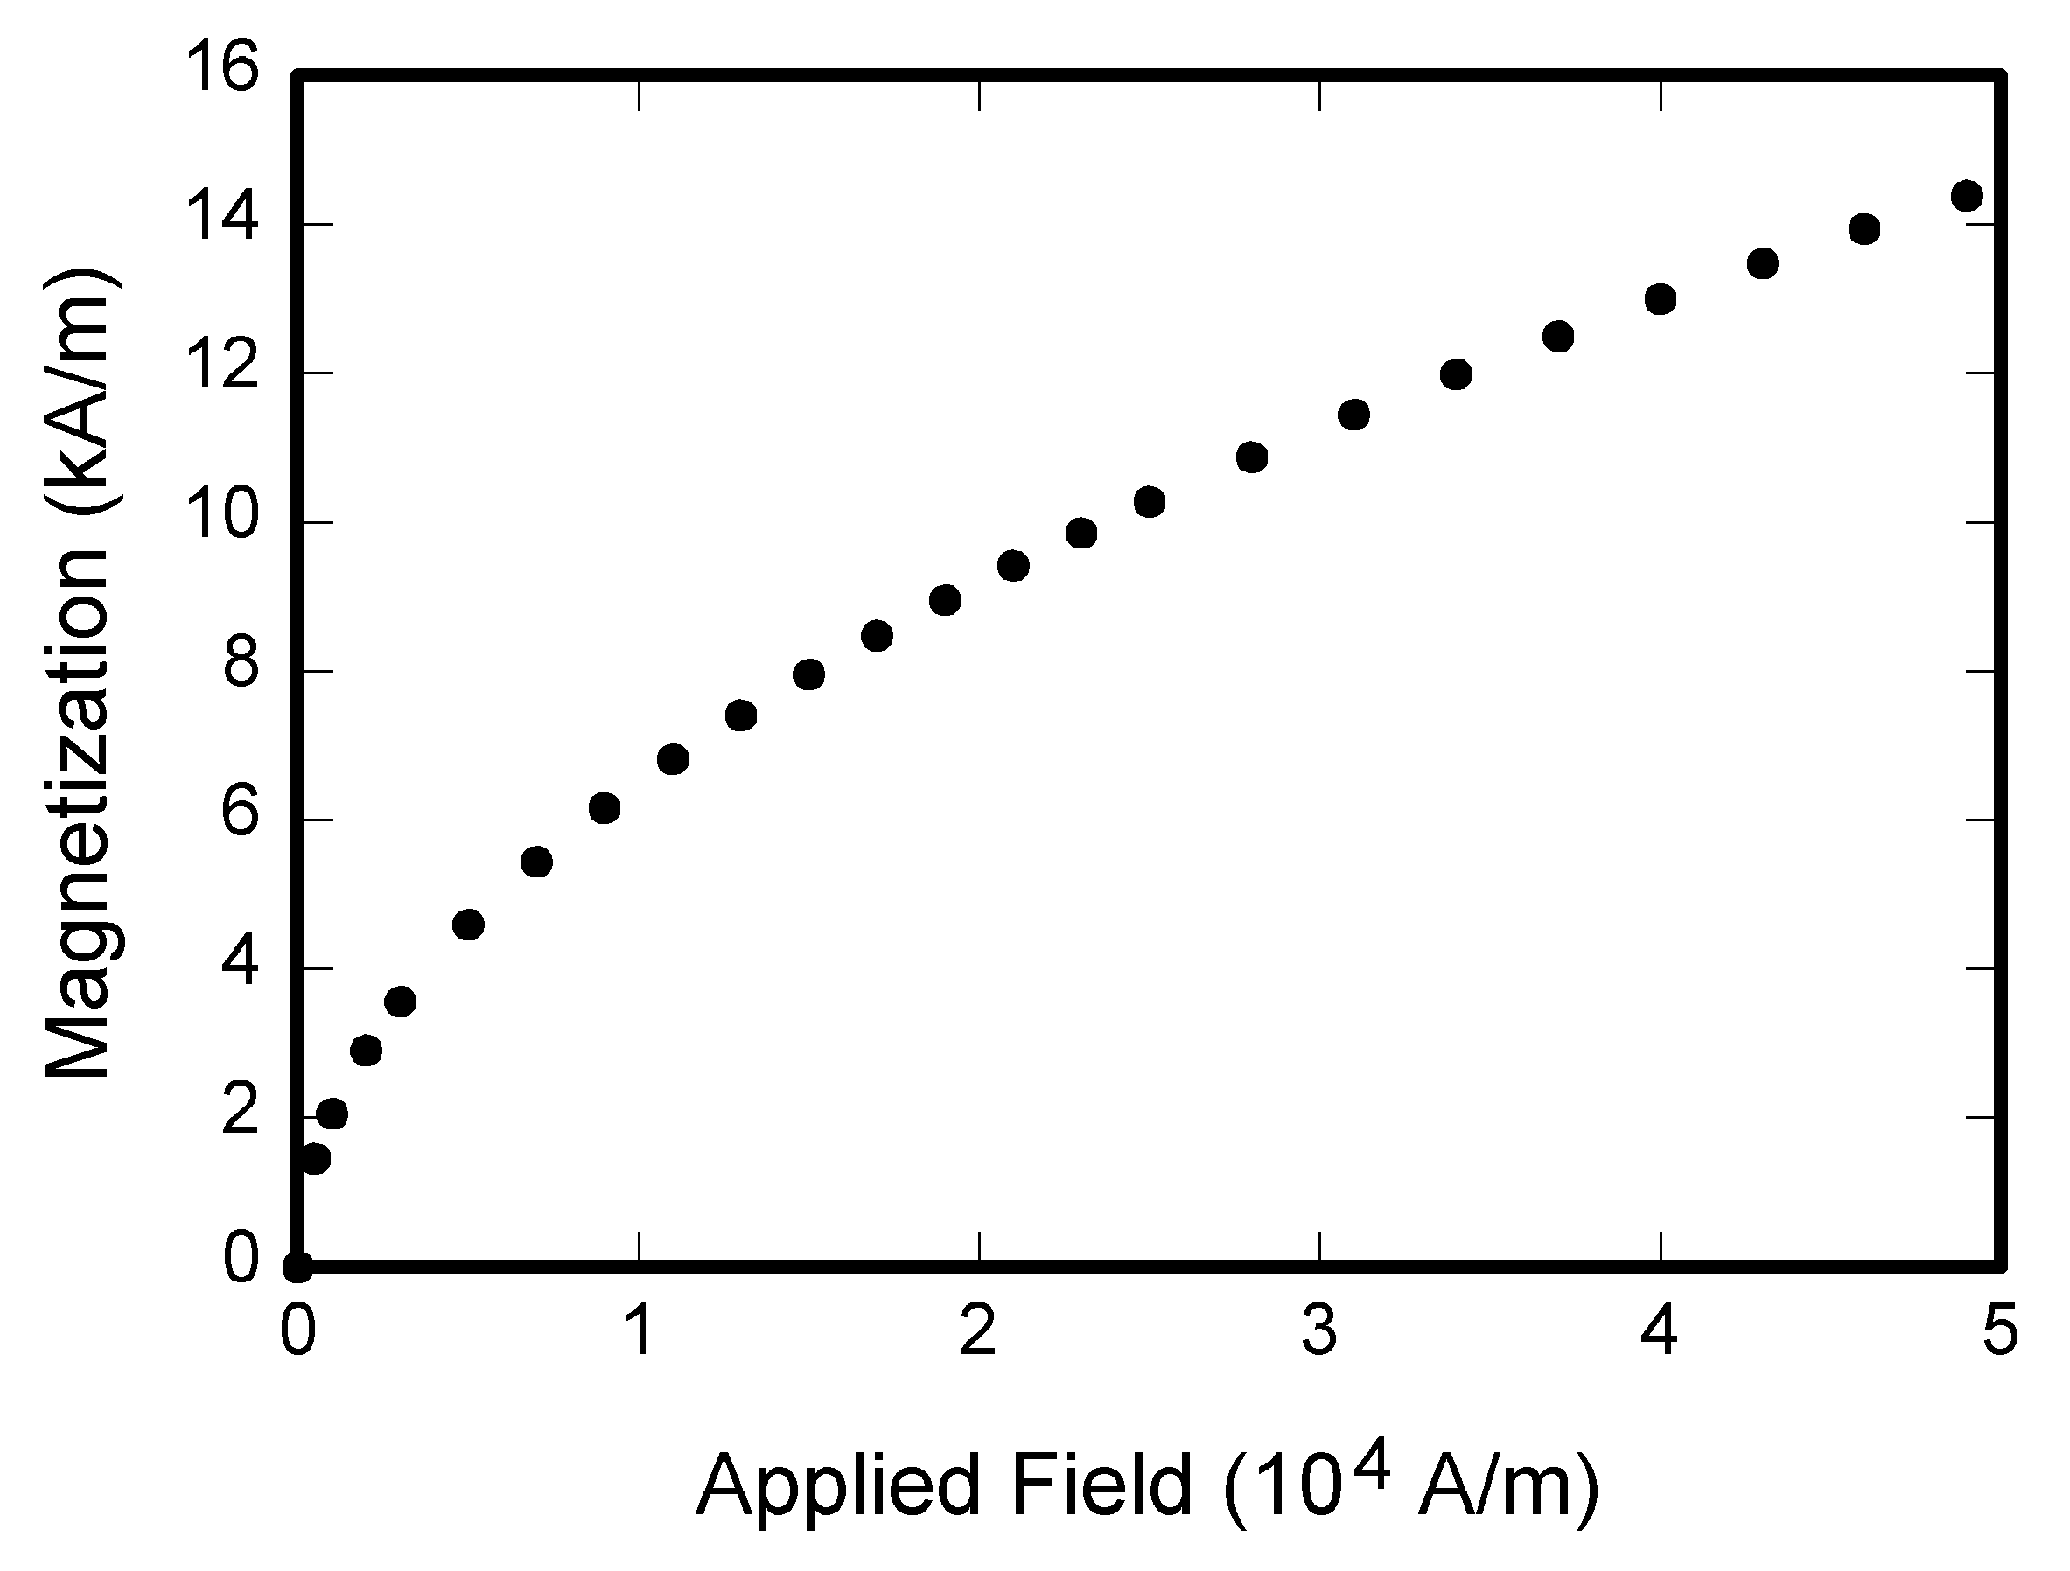
\includegraphics{fig1.png}}
% \caption{Example of a figure caption.}
% \label{fig}
% \end{figure}

% Figure Labels: Use 8 point Times New Roman for Figure labels. Use words 
% rather than symbols or abbreviations when writing Figure axis labels to 
% avoid confusing the reader. As an example, write the quantity 
% ``Magnetization'', or ``Magnetization, M'', not just ``M''. If including 
% units in the label, present them within parentheses. Do not label axes only 
% with units. In the example, write ``Magnetization (A/m)'' or ``Magnetization 
% \{A[m(1)]\}'', not just ``A/m''. Do not label axes with a ratio of 
% quantities and units. For example, write ``Temperature (K)'', not 
% ``Temperature/K''.

% \section*{Acknowledgment}

% The preferred spelling of the word ``acknowledgment'' in America is without 
% an ``e'' after the ``g''. Avoid the stilted expression ``one of us (R. B. 
% G.) thanks $\ldots$''. Instead, try ``R. B. G. thanks$\ldots$''. Put sponsor 
% acknowledgments in the unnumbered footnote on the first page.

% \begin{thebibliography}{00}
% \bibitem{b1} G. Eason, B. Noble, and I. N. Sneddon, ``On certain integrals of Lipschitz-Hankel type involving products of Bessel functions,'' Phil. Trans. Roy. Soc. London, vol. A247, pp. 529--551, April 1955.
% \bibitem{b2} J. Clerk Maxwell, A Treatise on Electricity and Magnetism, 3rd ed., vol. 2. Oxford: Clarendon, 1892, pp.68--73.
% \bibitem{b3} I. S. Jacobs and C. P. Bean, ``Fine particles, thin films and exchange anisotropy,'' in Magnetism, vol. III, G. T. Rado and H. Suhl, Eds. New York: Academic, 1963, pp. 271--350.
% \bibitem{b4} K. Elissa, ``Title of paper if known,'' unpublished.
% \bibitem{b5} R. Nicole, ``Title of paper with only first word capitalized,'' J. Name Stand. Abbrev., in press.
% \bibitem{b6} Y. Yorozu, M. Hirano, K. Oka, and Y. Tagawa, ``Electron spectroscopy studies on magneto-optical media and plastic substrate interface,'' IEEE Transl. J. Magn. Japan, vol. 2, pp. 740--741, August 1987 [Digests 9th Annual Conf. Magnetics Japan, p. 301, 1982].
% \bibitem{b7} M. Young, The Technical Writer's Handbook. Mill Valley, CA: University Science, 1989.
% \bibitem{b8} D. P. Kingma and M. Welling, ``Auto-encoding variational Bayes,'' 2013, arXiv:1312.6114. [Online]. Available: https://arxiv.org/abs/1312.6114
% \bibitem{b9} S. Liu, ``Wi-Fi Energy Detection Testbed (12MTC),'' 2023, gitHub repository. [Online]. Available: https://github.com/liustone99/Wi-Fi-Energy-Detection-Testbed-12MTC
% \bibitem{b10} ``Treatment episode data set: discharges (TEDS-D): concatenated, 2006 to 2009.'' U.S. Department of Health and Human Services, Substance Abuse and Mental Health Services Administration, Office of Applied Studies, August, 2013, DOI:10.3886/ICPSR30122.v2
% \bibitem{b11} K. Eves and J. Valasek, ``Adaptive control for singularly perturbed systems examples,'' Code Ocean, Aug. 2023. [Online]. Available: https://codeocean.com/capsule/4989235/tree
% \end{thebibliography}
\bibliographystyle{IEEEtran}
\bibliography{ref}

\vspace{12pt}
\color{red}
IEEE conference templates contain guidance text for composing and formatting conference papers. Please ensure that all template text is removed from your conference paper prior to submission to the conference. Failure to remove the template text from your paper may result in your paper not being published.

\end{document}
